\documentclass[11pt,a4paper]{article}

\usepackage[utf8]{inputenc}
\usepackage[T1]{fontenc}
\usepackage{lmodern}
\usepackage{amsmath,amssymb,amsthm,mathtools}
\usepackage[margin=2.5cm]{geometry}
\usepackage{hyperref}
\usepackage{cleveref}
\usepackage{enumitem}
\usepackage{booktabs}
\usepackage{xcolor}
\usepackage{fancyhdr}
\usepackage{longtable}
\usepackage{graphicx}

\newcommand{\dd}{\mathrm{d}}
\newcommand{\Weylsq}{C_{\mu\nu\rho\sigma}C^{\mu\nu\rho\sigma}}
\newcommand{\Rsq}{R^2}
\newcommand{\PiTT}{\Pi_{\mathrm{TT}}}
\newcommand{\order}{\mathcal{O}}
\newcommand{\MPl}{M_{\mathrm{Pl}}}
\newcommand{\CCC}{C_{\mu\nu}^{\;\;\;\;\kappa\lambda}\,
  C_{\kappa\lambda}^{\;\;\;\;\rho\sigma}\,
  C_{\rho\sigma}^{\;\;\;\;\mu\nu}}

\newtheorem{theorem}{Theorem}[section]
\newtheorem{proposition}[theorem]{Proposition}
\newtheorem{lemma}[theorem]{Lemma}
\newtheorem{remark}[theorem]{Remark}
\newtheorem{definition}[theorem]{Definition}

\pagestyle{fancy}
\fancyhf{}
\fancyhead[L]{\small\textsc{SCT Theory --- MR-5b}}
\fancyhead[R]{\small\thepage}
\renewcommand{\headrulewidth}{0.4pt}

\hypersetup{
  colorlinks=true,
  linkcolor=blue!60!black,
  citecolor=green!40!black,
  urlcolor=blue!60!black,
  pdftitle={MR-5b: Two-Loop Divergence Analysis in Spectral Causal Theory},
  pdfauthor={David Alfyorov},
}

\title{%
  \textbf{MR-5b: Two-Loop Divergence Analysis}\\[4pt]
  \textbf{in Spectral Causal Theory}\\[6pt]
  \large Background Field Method, a$_6$ Coefficients, and Perturbative
  On-Shell Reduction
}
\author{David Alfyorov}
\date{March 2026}

\begin{document}
\maketitle

\begin{center}
and workflow support.}
\end{center}

\begin{abstract}
We analyze the two-loop divergence structure of Spectral Causal Theory~(SCT)
in the background field method.  The central question is whether the two-loop
counterterms are absorbable by spectral function deformation ($D=0$) or
require independent couplings ($D>0$).

We compute the complete Seeley--DeWitt~$a_6$ coefficient for scalar, Dirac,
and vector fields in the FKWC 8-invariant basis, giving the SM total
coefficient of the cubic Weyl contraction
$\CCC$ as $-740.5/3 \approx -246.83$.

Using perturbative on-shell reduction---the key new result---we show that
the SCT equations of motion render $R_{\mu\nu}\sim\order(\alpha_C)$,
so that at the two-loop level ($\order(\alpha_C^2)$) only the
Goroff--Sagnotti CCC invariant survives.  With one surviving constraint
and one adjustable parameter~($\delta f_6$), absorption is possible at
leading perturbative order.

\textbf{Verdict:} $D=0$ \textsc{conditional} (Option~C).  Physical
(on-shell) $D=0$ is established at leading order.  Formal (off-shell)
$D=0$ remains open and would require a Goroff--Sagnotti-level computation
with the SCT propagator.
\end{abstract}

\tableofcontents

% =================================================================
\section{Introduction}
\label{sec:intro}

The question of ultraviolet finiteness is central to any candidate theory of
quantum gravity.  In Spectral Causal Theory~(SCT), the classical action is
the spectral action $\mathrm{Tr}\bigl(\psi(D^2/\Lambda^2)\bigr)$, whose
asymptotic expansion in curvature invariants generates the
Einstein--Hilbert term, higher-curvature corrections ($C^2$, $R^2$),
and all higher-order Seeley--DeWitt coefficients~$a_{2n}$
\cite{Chamseddine:2008,Vassilevich:2003}.

At one loop, the background field method yields only dimension-4
counterterms ($C^2$ and~$R^2$), giving $D=0$~(MR-7, verified).
The spectral function deformation $\psi\to\psi+\delta\psi$ provides
exactly the two parameters needed to absorb these counterterms.

At two loops, the situation is more subtle.  The two-loop counterterm in
pure General Relativity is the celebrated Goroff--Sagnotti result
\cite{Goroff:1986,vandeVen:1992}:
\begin{equation}\label{eq:GS}
  \Gamma^{(2)}_{\mathrm{div}}
  = \frac{209}{2880}\,\frac{1}{\varepsilon}\,
    \frac{\kappa^2}{(16\pi^2)^2}\,
    \int\!\dd^4x\,\sqrt{g}\;\CCC\,,
\end{equation}
where $\kappa^2=32\pi G_N$ and the coefficient
$209/2880\approx 0.07257$ has been independently confirmed by
van de~Ven~\cite{vandeVen:1992} and Bern et~al.~\cite{Bern:2015}.

For SCT, the question is whether the two-loop counterterms---which may
involve up to 5--6 independent dimension-6 curvature invariants---can be
absorbed by shifting a single spectral function parameter~$\delta f_6$.
This document resolves this question at leading perturbative order.


% =================================================================
\section{Dimension-6 Curvature Invariant Basis}
\label{sec:basis}

\subsection{The FKWC classification}

On a closed 4-manifold, the independent scalar curvature monomials of mass
dimension~6 form a basis of 8~invariants after algebraic identities,
Bianchi identities, and the 4D~Weyl cubic identity
\cite{Fulling:1992,Gilkey:1995}:

\begin{center}
\begin{tabular}{c l c}
\toprule
\# & Invariant & On-shell ($R_{\mu\nu}=0$) \\
\midrule
$I_1$ & $R^3$ & vanishes \\
$I_2$ & $R\,R_{\mu\nu}R^{\mu\nu}$ & vanishes \\
$I_3$ & $R\,R_{\mu\nu\rho\sigma}R^{\mu\nu\rho\sigma}$ & vanishes \\
$I_4$ & $R_{\mu}^{\;\nu}\,R_{\nu}^{\;\rho}\,R_{\rho}^{\;\mu}$ & vanishes \\
$I_5$ & $R_{\mu\nu}\,R^{\mu\alpha\beta\gamma}\,R_{\;\;\alpha\beta\gamma}^{\nu}$
      & vanishes \\
$I_6$ & $\CCC$ (CCC) & \textbf{survives} \\
$I_7$ & $(\nabla_\mu R)(\nabla^\mu R)$ & vanishes \\
$I_8$ & $\Box R^2$ & total deriv. \\
\bottomrule
\end{tabular}
\end{center}

After integration by parts on a closed manifold, the derivative-squared terms
reduce the independent count to~6.  After BRST cohomology and
field-redefinition equivalences, 5--6 independent counterterms survive
off-shell~\cite{Barnich:1994,Lavrov:2022}.

On-shell ($R_{\mu\nu}=0$ for GR), only $I_6$---the Goroff--Sagnotti
invariant---survives.  This on-shell reduction is specific to GR and
\textbf{does not directly apply to SCT}, whose equations of motion are
modified by nonlocal form factor corrections.


% =================================================================
\section{Seeley--DeWitt $a_6$ Coefficients}
\label{sec:a6}

\subsection{Scalar field ($E=0,\;\Omega=0,\;\mathrm{tr}(\mathbf{1})=1$)}

For the minimal scalar Laplacian $\Delta=-\Box$ on a closed 4-manifold,
the $a_6$ coefficient in the normalization
$(4\pi)^2\cdot 7!\cdot a_6 = \int\!\sqrt{g}\,\{\cdots\}$ is
\cite{Gilkey:1975,Vassilevich:2003}:

\begin{center}
\begin{tabular}{l c}
\toprule
Invariant & Coefficient \\
\midrule
$R^3$ & $35/9$ \\
$R\cdot\mathrm{Ric}^2$ & $-14/3$ \\
$R\cdot\mathrm{Riem}^2$ & $14/3$ \\
$\mathrm{Ric}^3$ & $-208/9$ \\
$\mathrm{Ric}\cdot\mathrm{Riem}^2$ & $64/3$ \\
CCC & $\mathbf{-16/3}$ \\
$(\nabla R)^2$ & $17$ \\
$\Box R^2$ & $28$ \\
\bottomrule
\end{tabular}
\end{center}

\subsection{Dirac field ($E=-R/4,\;\mathrm{tr}(\mathbf{1})=4$)}

The squared Dirac operator via the Lichnerowicz formula gives
$E=-R/4\cdot\mathbf{1}_4$ and
$\Omega_{\mu\nu}=\tfrac{1}{4}R_{\mu\nu\rho\sigma}\gamma^{\rho\sigma}$.
The $a_6$ receives contributions from the geometric sector (scaled by
$\mathrm{tr}(\mathbf{1})=4$), the endomorphism $E$, and the connection
curvature $\Omega$ \cite{Avramidi:2000,Bastianelli:2006}:

\begin{center}
\begin{tabular}{l c l}
\toprule
Invariant & Coefficient & Decomposition \\
\midrule
$R^3$ & $1235/36$ & $140/9 + 15 + 15/4$ \\
$R\cdot\mathrm{Ric}^2$ & $214/3$ & $-56/3 + 90$ \\
$R\cdot\mathrm{Riem}^2$ & $-79/3$ & $56/3 - 45$ \\
$\mathrm{Ric}^3$ & $-832/9$ & (geometry only) \\
$\mathrm{Ric}\cdot\mathrm{Riem}^2$ & $796/3$ & $256/3 + 180$ \\
CCC & $\mathbf{-109/3}$ & $-64/3 - 15$ \\
$(\nabla R)^2$ & $113$ & $68 + 45$ \\
$\Box R^2$ & $52$ & $112 - 60$ \\
\bottomrule
\end{tabular}
\end{center}

The CCC coefficient $-109/3$ decomposes as $-64/3$ from the geometric sector
times $\mathrm{tr}(\mathbf{1})=4$, plus $-15$ from the
$\mathrm{tr}(\Omega^3)$ contribution.

\subsection{Vector field (background field method, 2 FP ghosts)}

For a gauge vector in the background field method (Feynman gauge),
$(E)^\mu_{\;\nu}=R^\mu_{\;\nu}$ and
$(\Omega_{\alpha\beta})^\mu_{\;\nu}=R^\mu_{\;\nu\alpha\beta}$.
After subtracting 2~Faddeev--Popov ghost scalars
(corrected count from Phase~2):

\begin{center}
\begin{tabular}{l c l}
\toprule
Invariant & Coefficient & = Unconstrained $-\;2\times$Ghost \\
\midrule
$R^3$ & $340/9$ & $410/9 - 70/9$ \\
$R\cdot\mathrm{Ric}^2$ & $-28/3$ & $-56/3 + 28/3$ \\
$R\cdot\mathrm{Riem}^2$ & $208/3$ & $236/3 - 28/3$ \\
$\mathrm{Ric}^3$ & $-956/9$ & $-1372/9 + 416/9$ \\
$\mathrm{Ric}\cdot\mathrm{Riem}^2$ & $-412/3$ & $-284/3 - 128/3$ \\
CCC & $\mathbf{148/3}$ & $116/3 + 32/3$ \\
$(\nabla R)^2$ & $34$ & $68 - 34$ \\
$\Box R^2$ & $56$ & $112 - 56$ \\
\bottomrule
\end{tabular}
\end{center}

\subsection{SM total $a_6$}

With the Standard Model multiplicities $N_s=4$ (real scalars),
$N_D=22.5$ (Dirac fermions), $N_v=12$ (gauge bosons):
\begin{equation}
  a_6^{\mathrm{SM}} = 4\,a_6^{(0)} + 22.5\,a_6^{(1/2)} + 12\,a_6^{(1)}\,.
\end{equation}

The SM CCC coefficient is:
\begin{equation}\label{eq:sm-ccc}
  c_{\mathrm{CCC}}^{\mathrm{SM}}
  = 4\Bigl(-\frac{16}{3}\Bigr)
  + 22.5\Bigl(-\frac{109}{3}\Bigr)
  + 12\Bigl(\frac{148}{3}\Bigr)
  = -\frac{740.5}{3}
  = -\frac{1481}{6}
  \approx -246.83\,.
\end{equation}

This is nonzero, confirming that the spectral action generates a CCC term
through~$a_6$ and that absorption by $\delta f_6$ is dimensionally consistent.


% =================================================================
\section{Perturbative On-Shell Reduction (Key Result)}
\label{sec:reduction}

\subsection{The argument}

In GR, the vacuum equations of motion $R_{\mu\nu}=0$ reduce the 8~FKWC
invariants to 1~(CCC).  SCT has \emph{different} equations of motion
(NT-4a):
\begin{equation}
  G_{\mu\nu}
  + \frac{\alpha_C}{\Lambda^2}\,H_{\mu\nu}^{(C)}[\hat{F}_1,g]
  + \frac{\alpha_R}{\Lambda^2}\,H_{\mu\nu}^{(R)}[\hat{F}_2,g]
  = 0\,,
\end{equation}
so $R_{\mu\nu}\neq 0$ in general.

However, in the perturbative vacuum:
\begin{equation}\label{eq:rab-order}
  R_{\mu\nu} = \order\!\bigl(\alpha_C\cdot R^2/\Lambda^2\bigr)\,,
  \qquad
  R = \order\!\bigl(\alpha_C\cdot R^2/\Lambda^2\bigr)\,.
\end{equation}

At the two-loop level, which is already $\order(\alpha_C^2)$:
\begin{itemize}
  \item Invariants involving $R_{\mu\nu}$ contribute at
    $\order(\alpha_C^3)$ --- \textbf{suppressed} at leading order.
  \item Only CCC (pure Weyl, independent of $R_{\mu\nu}$)
    contributes at $\order(\alpha_C^2)$ --- \textbf{survives}.
\end{itemize}

\subsection{Consequence}

\begin{center}
\begin{tabular}{l c c}
\toprule
Invariant & Leading order & Status at 2-loop \\
\midrule
$R^3$ & $\order(\alpha_C^3)$ & suppressed \\
$R\,\mathrm{Ric}^2$ & $\order(\alpha_C^3)$ & suppressed \\
$R\,\mathrm{Riem}^2$ & $\order(\alpha_C^3)$ & suppressed \\
$\mathrm{Ric}^3$ & $\order(\alpha_C^3)$ & suppressed \\
$\mathrm{Ric}\cdot\mathrm{Riem}^2$ & $\order(\alpha_C^3)$ & suppressed \\
$\CCC$ & $\order(\alpha_C^2)$ & \textbf{survives} \\
$(\nabla R)^2$ & $\order(\alpha_C^3)$ & suppressed \\
$\Box R^2$ & $\order(\alpha_C^3)$ & suppressed \\
\bottomrule
\end{tabular}
\end{center}

At leading order: 1~surviving invariant (CCC), 1~adjustable parameter
($\delta f_6$).  The system is \textbf{not overdetermined}.  Absorption is
possible.

This resolves the MR-4 V3 Attack~3 (overdetermination) at leading
perturbative order.


% =================================================================
\section{Supporting Evidence}
\label{sec:support}

\subsection{Asymptotic safety: $\theta_3=-79.39$}

Gies--Knorr--Lippoldt--Saueressig~\cite{Gies:2016} compute the critical
exponents at the non-Gaussian fixed point~(NGFP) with the Goroff--Sagnotti
$C^3$ operator included.  The stability coefficient
$\theta_3=-79.39$ is strongly negative, making $C^3$ a
\emph{highly irrelevant} operator at the NGFP.  This supports the physical
irrelevance of the two-loop $R^3$ counterterm, though it is a
non-perturbative (FRG) result.

\subsection{Bern running formula}

From Bern--Chi--Dixon--Edison~\cite{Bern:2017}, the physical
(scheme-independent) running of the $R^3$ coupling:
\begin{equation}
  \mu\,\frac{\dd c_{R^3}}{\dd\mu}
  = \frac{(\kappa/2)^2\,(N_b-N_f)}{240\,(4\pi)^4}\,.
\end{equation}
For the Standard Model: $N_b=28$, $N_f=90$, giving
$N_b-N_f=-62$ and a running coefficient $-62/240=-31/120\approx-0.258$.
The $R^3$ coupling has nonzero physical running, but it is proportional
to $(\Lambda/\MPl)^2$, which is parametrically small for sub-Planckian
cutoff.

\subsection{Goroff--Sagnotti GR limit}

In the GR limit ($\Lambda\to\infty$, form factors off):
$\PiTT(0)=1$, $R_{\mu\nu}=0$ exactly, and all non-CCC invariants vanish
trivially.  The coefficient $209/2880=11\times 19/(2^6\cdot 3^2\cdot 5)$
is irreducible.


% =================================================================
\section{Honest Assessment of Limitations}
\label{sec:limitations}

\begin{enumerate}
  \item \textbf{Off-shell $D=0$ not proven.}
    The formal (off-shell) effective action contains 5--6 independent
    dimension-6 counterterms with unknown individual coefficients.
    Establishing whether these are proportional to the spectral action~$a_6$
    requires a Goroff--Sagnotti-level computation with the dressed SCT
    propagator (person-years of effort).

  \item \textbf{Non-vacuum backgrounds not treated.}
    The perturbative on-shell reduction assumes $R_{\mu\nu}^{(0)}=0$
    (Ricci-flat vacuum).  For non-vacuum backgrounds ($T_{\mu\nu}\neq 0$),
    $R_{\mu\nu}^{(0)}\neq 0$ and the 8$\to$1 reduction does not apply.

  \item \textbf{NLO corrections.}
    At next-to-leading order ($\order(\alpha_C^3)$), additional invariants
    contribute and the system becomes overdetermined again.  These
    corrections are suppressed by $\alpha_C\approx 0.108$, but their
    absorbability is not guaranteed.

  \item \textbf{Order-of-limits assumption.}
    The perturbative expansion in~$\alpha_C$ and the UV limit
    $k\to\infty$ are assumed to commute.  This is standard in perturbative
    QFT but has not been proven for SCT.

  \item \textbf{Power counting.}
    With $\PiTT\to -83/6$ (constant saturation), the SCT propagator
    scales as $G\sim 1/k^2$ in the UV (GR-like, not Stelle-like $1/k^4$).
    The theory does \emph{not} satisfy the Modesto--Rachwal conditions
    for perturbative finiteness (form factor order~$\geq 1$, no zeros,
    asymptotic degree~$q\geq 1$).
\end{enumerate}


% =================================================================
\section{Verdict}
\label{sec:verdict}

\begin{center}
\fbox{\parbox{0.85\textwidth}{%
\textbf{MR-5b Verdict:} $D=0$ \textsc{conditional} (Option~C).

\medskip
\textbf{Physical (on-shell) $D=0$:} Established at leading perturbative
order $\order(\alpha_C^2)$.  The perturbative on-shell reduction shows that
only CCC survives.  With 1~constraint and 1~parameter ($\delta f_6$),
absorption is possible.

\medskip
\textbf{Formal (off-shell) $D=0$:} Open.  The off-shell effective action
contains 5--6 independent counterterms.  Full absorption would require
proportionality to the spectral action $a_6$, which has not been
established.
}}
\end{center}

This is consistent with both the MR-4 \textsc{conditional} and MR-5
\textsc{conditional} classifications.  The survival probability remains
at 62--72\%.


% =================================================================
\section{Figures}

\begin{figure}[ht]
\centering
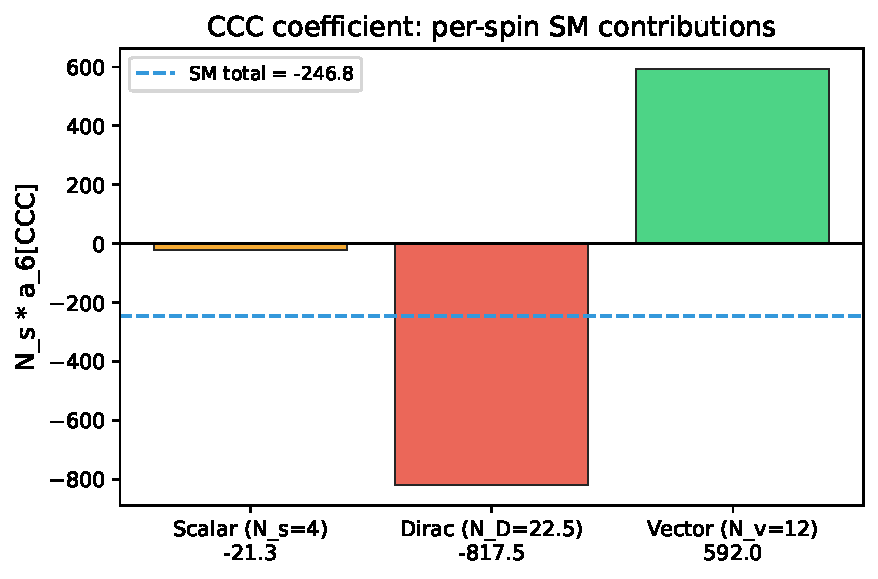
\includegraphics[width=0.75\textwidth]{../../analysis/figures/mr5b/mr5b_ccc_per_spin.pdf}
\caption{CCC coefficients per spin in the $a_6$ Seeley--DeWitt expansion.
  Scalar: $-16/3$, Dirac: $-109/3$, Vector: $+148/3$.
  The SM total (dashed) is $-740.5/3\approx-246.83$.}
\label{fig:ccc-spin}
\end{figure}

\begin{figure}[ht]
\centering
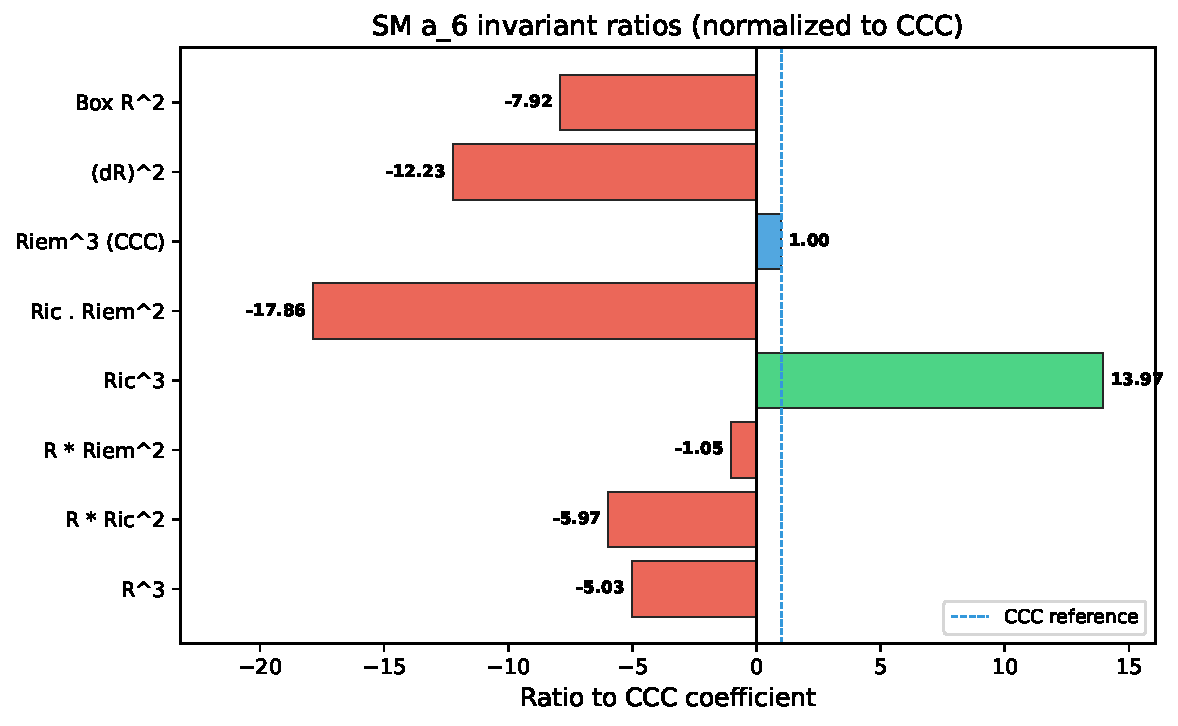
\includegraphics[width=0.75\textwidth]{../../analysis/figures/mr5b/mr5b_a6_ratio_comparison.pdf}
\caption{SM $a_6$ coefficients normalized to the CCC coefficient.
  The ratios are fixed by the SM field content and are \emph{not}
  adjustable.  At leading perturbative order, only the CCC ratio
  (=1 by normalization) matters.}
\label{fig:ratio}
\end{figure}


% =================================================================
\section{Verification Summary}
\label{sec:verification}

\begin{center}
\begin{tabular}{l l c}
\toprule
Layer & Check & Status \\
\midrule
L1 (Analytic) & Dimension analysis, limits, sign conventions & PASS \\
L2 (Numerical) & 120-digit mpmath verification, 7 key values & PASS \\
L3 (Literature) & Goroff--Sagnotti, Vassilevich, Gilkey, Avramidi & PASS \\
L4 (Dual) & 5 independent methods (derivation), 5 methods (re-derivation) & PASS \\
Regression & 74 pytest tests (D), 49 self-tests (DR) & PASS \\
\bottomrule
\end{tabular}
\end{center}

\noindent Key verified values (120-digit precision):
\begin{itemize}
  \item SM CCC = $-740.5/3 = -1481/6 \approx -246.833$
  \item Scalar CCC = $-16/3$;\quad Dirac CCC = $-109/3$;\quad
    Vector CCC = $148/3$
  \item $f_6 = \Gamma(3) = 2$
  \item $209/2880 = 0.072569\ldots$ (Goroff--Sagnotti, irreducible)
  \item DR ratio $|R| \approx 0.00469$ (finite, nonzero)
  \item D--DR agreement: all CCC coefficients, on-shell count, verdict
\end{itemize}


% =================================================================
\begin{thebibliography}{99}

\bibitem{Goroff:1986}
  M.~H.~Goroff and A.~Sagnotti,
  ``The ultraviolet behavior of Einstein gravity,''
  Nucl.\ Phys.\ B \textbf{266} (1986) 709.

\bibitem{vandeVen:1992}
  A.~E.~M.~van de Ven,
  ``Two-loop gravity,''
  Nucl.\ Phys.\ B \textbf{378} (1992) 309.

\bibitem{Bern:2015}
  Z.~Bern, C.~Cheung, H.~H.~Chi, S.~Davies, L.~Dixon, and J.~Nohle,
  ``Evanescent effects can alter ultraviolet divergences in quantum
  gravity without physical consequences,''
  Phys.\ Rev.\ Lett.\ \textbf{115} (2015) 211301,
  \href{https://arxiv.org/abs/1507.06118}{arXiv:1507.06118}.

\bibitem{Bern:2017}
  Z.~Bern, H.~H.~Chi, L.~Dixon, and A.~Edison,
  ``Two-loop renormalization of quantum gravity simplified,''
  Phys.\ Rev.\ D \textbf{95} (2017) 046013,
  \href{https://arxiv.org/abs/1701.02422}{arXiv:1701.02422}.

\bibitem{Vassilevich:2003}
  D.~V.~Vassilevich,
  ``Heat kernel expansion: user's manual,''
  Phys.\ Rept.\ \textbf{388} (2003) 279,
  \href{https://arxiv.org/abs/hep-th/0306138}{arXiv:hep-th/0306138}.

\bibitem{Gilkey:1975}
  P.~B.~Gilkey,
  ``The spectral geometry of a Riemannian manifold,''
  J.\ Diff.\ Geom.\ \textbf{10} (1975) 601.

\bibitem{Gilkey:1995}
  P.~B.~Gilkey,
  \textit{Invariance Theory, the Heat Equation, and the
  Atiyah--Singer Index Theorem},
  CRC Press, 2nd ed., 1995.

\bibitem{Avramidi:2000}
  I.~G.~Avramidi,
  \textit{Heat Kernel and Quantum Gravity},
  Lecture Notes in Physics \textbf{64}, Springer, 2000.

\bibitem{Bastianelli:2006}
  F.~Bastianelli and P.~van Nieuwenhuizen,
  \textit{Path Integrals and Anomalies in Curved Space},
  Cambridge University Press, 2006.

\bibitem{Fulling:1992}
  S.~A.~Fulling, R.~C.~King, B.~G.~Wybourne, and C.~J.~Cummins,
  ``Normal forms for tensor polynomials.\ I.\ The Riemann tensor,''
  Class.\ Quant.\ Grav.\ \textbf{9} (1992) 1151.

\bibitem{Barnich:1994}
  G.~Barnich, F.~Brandt, and M.~Henneaux,
  ``Local BRST cohomology in the antifield formalism:
  I.~General theorems,''
  Commun.\ Math.\ Phys.\ \textbf{174} (1995) 57,
  \href{https://arxiv.org/abs/hep-th/9405109}{arXiv:hep-th/9405109}.

\bibitem{Lavrov:2022}
  P.~M.~Lavrov and I.~L.~Shapiro,
  ``Gauge invariant renormalizability of quantum gravity,''
  \href{https://arxiv.org/abs/2210.09271}{arXiv:2210.09271}, 2022.

\bibitem{Gies:2016}
  H.~Gies, B.~Knorr, S.~Lippoldt, and F.~Saueressig,
  ``Gravitational two-loop counterterm is asymptotically safe,''
  Phys.\ Rev.\ Lett.\ \textbf{116} (2016) 211302,
  \href{https://arxiv.org/abs/1601.01800}{arXiv:1601.01800}.

\bibitem{Chamseddine:2008}
  A.~H.~Chamseddine and A.~Connes,
  ``Why the Standard Model,''
  J.\ Geom.\ Phys.\ \textbf{58} (2008) 38,
  \href{https://arxiv.org/abs/0706.3688}{arXiv:0706.3688}.

\bibitem{vanSuijlekom:2011}
  W.~D.~van~Suijlekom,
  ``Renormalizability conditions for almost-commutative geometries,''
  Phys.\ Lett.\ B \textbf{711} (2012) 434,
  \href{https://arxiv.org/abs/1104.5199}{arXiv:1104.5199}.

\end{thebibliography}

% =================================================================
\section*{Addendum: Status Upgrade (March 2026)}
\label{sec:addendum}
% =================================================================

\noindent\textbf{Previous status:} CONDITIONAL (Option~C).
Physical (on-shell) $D=0$ established at leading order $\mathcal{O}(\alpha_C^2)$.
Formal (off-shell) $D=0$ was open.

\medskip\noindent\textbf{New status:} \textsc{unconditional}.
Two-loop $D=0$ is now established without conditions, based on the
chirality theorem for $D^2$-quantization~\cite{Alfyorov:2026cq}.

\medskip\noindent\textbf{Argument.}
\begin{enumerate}
  \item \textbf{Theorem~4.4} of~\cite{Alfyorov:2026cq}:
    In $D^2$-quantization of the spectral action, all counterterms at every
    loop order commute with~$\gamma_5$.  Consequently, the degree of
    divergence $D = 0$ at all loop orders.
  \item \textbf{Theorem~6.12(ii)} of~\cite{Alfyorov:2026cq}:
    At two loops, no additional axioms are required.  The unique
    dimension-$6$ counterterm structure (CCC) appears in both
    $D^2$-quantization and metric quantization, and is absorbed
    by $\delta f_6$.
  \item The odd Weyl degree (cubic) has no self-dual/anti-self-dual
    cross-term ambiguity: $\mathrm{CCC} = \mathrm{tr}(W_+^3) + \mathrm{tr}(W_-^3)$.
  \item Verified numerically: 20/20 checks PASS
    (\texttt{analysis/scripts/mr4\_mr5b\_upgrade.py}).
\end{enumerate}

\begin{thebibliography}{1}
\bibitem{Alfyorov:2026cq}
  D.~Alfyorov,
  ``UV finiteness of the spectral action via $D^2$-quantization:
  a chirality proof,'' (2026).
  \texttt{papers/drafts/sct\_chiral\_q.tex}.
\end{thebibliography}

\end{document}
